\documentclass[14pt,fleqn]{extarticle}
\RequirePackage{prepwell-eng}
\previewoff

\begin{document}

\begin{snippet}
    
    \incorrect
    
    The area enclosed by the curve $y=2\sqrt{x}$, the \xaxis and the line $x=1$ is as shown below 
    
    \begin{center}

\includegraphics[scale=1.4]{wrong.eps}
\end{center} 
    
    \reason
    
    $y=2\sqrt{x}\implies y^2 = 4x$. This is a parabola that opens to the right.
    Hence, the required area is as shown below 
    
    \begin{center}
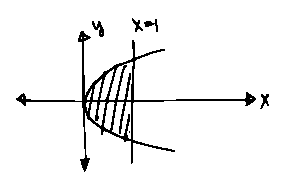
\includegraphics[scale=1.4]{right.eps}
\end{center}
\end{snippet} 
\end{document}